\beginsupplement

\newpage

\appendix

\section*{Appendix}

\section{Self-organizing maps}\label{sec:SOMs}

The general idea of a self-organizing map (SOM) is to approximate a data manifold in a high-dimensional continuous space with a lower dimensional discrete one \citep{Kohonen1998}.
It can therefore be seen as a nonlinear discrete dimensionality reduction.
The mapping is achieved by a procedure in which this discrete representation (the \emph{map}) is randomly embedded into the data space and then iteratively optimized to approach the data manifold more closely.

The map consists of $k$ nodes $V=\{v_1, \dots , v_k\}$, where every node corresponds to an embedding in the data space $e_v \in \mathbb{R}^d$ and a representation in the lower-dimensional discrete space $m_v \in M$, where usually $M \subset \mathbb{N}^2$.
There are two different geometrical measures that have to be considered during training: the neighborhood function $N(m_u, m_{\tilde{v}})$ that is defined on the low-dimensional map space and the Euclidean distance $D (e_u, e_{\tilde{v}}) = \| e_u - e_{\tilde{v}} \|_2$ in the high-dimensional data space.
The SOM optimization tries to induce a coupling between these two properties, such that the topological structure of the representation reflects the geometrical structure of the data.


\begin{algorithm}
\caption{Self-organizing map training}
\label{alg:som_train}

\begin{algorithmic}
	\Require data set $\mathcal{D} = \{x_1, \dots ,x_n \; \vert \; x_i \in \mathbb{R}^d\}$, number of nodes $k$, neighborhood function $N(\cdot)$, step size $\eta$
	\State initialize set of $k$ nodes $V=\{v_1, \dots , v_k\}$
	\State initialize embeddings $e_v \in \mathbb{R}^d \; \forall \; v \in V$
	\While{not converged}
	\ForAll {$x_i \in \mathcal{D}$}
		\State find the closest SOM node $\tilde{v} := \argmin_{v \in V} \| x_i - e_v \|_2$
		\State update node embedding $e_{\tilde{v}} \gets e_{\tilde{v}} + \eta \, (x_i - e_{\tilde{v}})$
		\ForAll {$u \in V \backslash \tilde{v}$}
			\State update neighbor embedding $e_u \gets e_u + \eta \, N(m_{\tilde{v}}, m_u) (x_i - e_u)$
		\EndFor
	\EndFor
	\EndWhile
\end{algorithmic}
	
\end{algorithm}

The SOM training procedure is described in Algorithm~\ref{alg:som_train}.
During training on a data set $\mathcal{D}$, a winner node $\tilde{v}$ is chosen for every point $x_i$ according to the Euclidean distance of the point and the node's embedding in the data space.
The embedding vector for the winner node is then updated by pulling it into the direction of the data point with some step size $\eta$.
The embedding vectors of the other nodes are also updated -- potentially with a smaller step size -- depending on whether they are neighbors of the winner node in the map space $M$.

The neighborhood is defined by the neighborhood function $N(m_u, m_{\tilde{v}})$.
There can be different design choices for the neighborhood function, e.g.\ rectangular grids, hexagonal grids or Gaussian neighborhoods.
For simplicity and ease of visualization, we usually choose a two-dimensional rectangular grid neighborhood in this paper.

In this original formulation of the SOM training, the nodes are updated one by one with a fixed step size.
In our model, however, we use a gradient-based optimization of their distances to the data points and update them in minibatches.
This leads to larger step sizes when they are farther away from the data and smaller step sizes when they are close.
Overall, our gradient-based SOM training seems to perform better than the original formulation (see Tab.~\ref{tab:performance}).

It also becomes evident from this procedure that it will be very hard for the map to fit disjoint manifolds in the data space.
Since the nodes of the SOM form a fully connected graph, they do not possess the ability to model spatial gaps in the data.
We overcome this problem in our work by mapping the data manifold with a variational autoencoder into a lower-dimensional latent space.
The VAE can then learn to close the aforementioned gaps and map the data onto a compact latent manifold, which can be more easily modeled with the SOM.



\section{Implementation details}\label{sec:implementation}

The hyperparameters of our model were optimized using Robust Bayesian Optimization with the packages \texttt{sacred} and \texttt{labwatch} \citep{Greff2017a} for the parameter handling and \texttt{RoBo} \citep{Klein2017} for the optimization, using the mean squared reconstruction error as the optimization criterion.
Especially the weighting hyperparameters $\alpha, \beta, \gamma$ and $\tau$ (see Eq.~\eqref{eq:L_somvae} and Eq.~\eqref{eq:L_prob}) have to be tuned carefully, such that the different parts of the model converge at roughly the same rate.
We found that 2000 steps of Bayesian optimization sufficed to yield a performant hyperparameter assignment.

Since our model defines a general framework, some competitor models can be seen as special cases of our model, where certain parts of the loss function are set to zero or parts of the architecture are omitted.
We used the same hyperparameters for those models.
For external competitor methods, we used the hyperparameters from the respective publications where applicable and otherwise the default parameters from their packages.
The models were implemented in TensorFlow \citep{GoogleResearch2015} and optimized using Adam \citep{Kingma2015}.


\section{Clustering performance measures}\label{sec:clustering_performance}

Given that one of our most interesting tasks at hand is the clustering of data, we need some performance measures to objectively compare the quality of this clustering with other methods.
The measures that we decided to use and that have been used extensively in the literature are \emph{purity} and \emph{normalized mutual information} (NMI) \citep{Manning2008}.
We briefly review them in the following.

Let the set of ground truth classes in the data be $C = \{ c_1, c_2, \dots, c_J \}$ and the set of clusters that result from the algorithm $\Omega = \{ \omega_1, \omega_2, \dots, \omega_K \}$.
The \emph{purity} $\pi$ is then defined as $\pi(C, \Omega) = \frac{1}{N} \sum_{k = 1}^K \max_j \vert \omega_k \cap c_j \vert$ where $N$ is the total number of data points.
Intuitively, the purity is the accuracy of the classifier that assigns the most prominent class label in each cluster to all of its respective data points.

While the purity has a very simple interpretation, it also has some shortcomings.
One can for instance easily observe that a clustering with $K = N$, i.e.\ one cluster for every single data point, will yield a purity of $1.0$ but still probably not be very informative for most tasks.
It would therefore be more sensible to have another measure that penalizes the number of clusters.
The normalized mutual information is one such measure.

The NMI is defined as $\textit{NMI}(C, \Omega) = \frac{2 \; I(C, \Omega)}{H(C) + H(\Omega)}$ where $I(C, \Omega)$ is the mutual information between $C$ and $\Omega$ and $H(\cdot)$ is the Shannon information entropy.
While the entropy of the classes is a data-dependent constant, the entropy of the clustering increases with the number of clusters.
It can therefore be seen as a penalty term to regularize the trade-off between low intra-cluster variance and a small number of clusters.
Both NMI and purity are normalized, i.e.\ take values in $[0,1]$.



\section{Experimental details}


\subsection{Clustering on MNIST and Fashion-MNIST} \label{sec:mnist_appendix}

Additionally to the results in Table~\ref{tab:performance}, we performed experiments to assess the influence of the number of clusters $k$ on the clustering performance of our method.
We chose different values for $k$ between 4 and 64 and tested the clustering performance on MNIST and Fashion-MNIST (Tab.~\ref{tab:k_performance}).

\begin{table}
    \centering
    \caption{Performance comparison of our method with different numbers of clusters in terms of purity and normalized mutual information on different benchmark data sets. The values are the means of 10 runs and the respective standard errors.}
    \begin{tabular}{lrrrr}
        \toprule
         & \multicolumn{2}{c}{MNIST} & \multicolumn{2}{c}{Fashion-MNIST} \\
        \cmidrule(rl){2-3}
        \cmidrule(rl){4-5}
        Number of clusters & \multicolumn{1}{c}{Purity} & \multicolumn{1}{c}{NMI} & \multicolumn{1}{c}{Purity} & \multicolumn{1}{c}{NMI} \\
         \midrule
         $k = 4$ & 0.364 $\pm$ 0.009 & 0.378 $\pm$ 0.018 & 0.359 $\pm$ 0.005 & 0.431 $\pm$ 0.008\\
         $k = 9$ & 0.626 $\pm$ 0.006 & 0.554 $\pm$ 0.004 & 0.558 $\pm$ 0.007 & 0.560 $\pm$ 0.006\\
         $k = 16$ & 0.721 $\pm$ 0.006 & 0.587 $\pm$ 0.003 & 0.684 $\pm$ 0.003 & \textbf{0.589 $\pm$ 0.003}\\
         $k = 25$ & 0.803 $\pm$ 0.003 & \textbf{0.613 $\pm$ 0.002} & 0.710 $\pm$ 0.003 & 0.572 $\pm$ 0.002\\
         $k = 36$ & 0.850 $\pm$ 0.002 & \textbf{0.612 $\pm$ 0.001} & 0.732 $\pm$ 0.002 & 0.556 $\pm$ 0.002\\
         $k = 49$ & 0.875 $\pm$ 0.002 & 0.608 $\pm$ 0.001 & 0.750 $\pm$ 0.002 & 0.545 $\pm$ 0.001\\
         $k = 64$ & \textbf{0.894 $\pm$ 0.002} & 0.599 $\pm$ 0.001 & \textbf{0.758 $\pm$ 0.002} & 0.532 $\pm$ 0.001\\
         \bottomrule
    \end{tabular}
    \label{tab:k_performance}
\end{table}

It can be seen that the purity increases monotonically with $k$, since it does not penalize larger numbers of clusters (see Sec.~\ref{sec:clustering_performance}).
The NMI, however, includes an automatic penalty for misspecifying the model with too many clusters.
It therefore increases first, but then decreases again for too large values of $k$.
The optimal $k$ according to the NMI seems to lie between 16 and 36.


\subsection{Interpretable representations of chaotic time series}\label{sec:lorenz_appendix}

The Lorenz system is the system of coupled ordinary differential equations defined by
%
\begin{equation*}
	\frac{dX}{dt} = a (Y - X) \hskip 4em
	\frac{dY}{dt} = X (b - Z) - Y \hskip 4em
	\frac{dZ}{dt} = XY - cZ
\end{equation*}
%
with tuning parameters $a$, $b$ and $c$. For parameter choices $a = 10$, $b = 28$ and $c = \frac{8}{3}$, the system shows chaotic behavior by forming a strange attractor \citep{Tucker1999} with the two attractor points being given by $p_{1,2} = \lbrack \pm \sqrt{c (b-1)}, \pm \sqrt{c (b-1)}, b-1 \rbrack^T$.

We simulated 100 trajectories of 10,000 time steps each from the chaotic system and trained the SOM-VAE as well as k-means on it with 64 clusters/embeddings respectively.
The system chaotically switches back and forth between the two attractor basins.
By computing the Euclidian distance between the current system state and each of the attractor points $p_{1,2}$, we can identify the current attractor basin at each time point.

In order to assess the interpretability of the learned representations, we have to define an objective measure of interpretability.
We define interpretability as the similarity between the representation and the system's ground truth macro-state.
Since representations at single time points are meaningless with respect to this measure, we compare the evolution of representations and system state over time in terms of their entropy.

We divided the simulated trajectories from our test set into spans of 100 time steps each.
For every subtrajectory, we computed the entropies of those subtrajectories in the real system space (macro-state and noise), the assigned attractor basin space (noise-free ground-truth macro-state), the SOM-VAE representation and the k-means representation.
We also observed for every subtrajectory whether or not a change between attractor basins has taken place.
Note that the attractor assignments and representations are discrete, while the real system space is continuous.
In order to make the entropies comparable, we discretize the system space into unit hypercubes for the entropy computation.
For a representation $\mathcal{R}$ with assignments $\mathcal{R}_t$ at time $t$ and starting time $t_{start}$ of the subtrajectory, the entropies are defined as
%
\begin{equation}
	H \left( \mathcal{R}, t_{start} \right) = H \left( \lbrace R_t \; \vert \; t_{start} \leq t < t_{start} + 100 \rbrace \right)
\end{equation}
%
with $H(\cdot)$ being the Shannon information entropy of a discrete set.


\subsection{Learning representations of acute physiological states in the ICU}\label{sec:ICU_appendix}

All experiments were performed on dynamic data extracted from the \texttt{eICU} Collaborative Research Database \citep{Goldberger2000}.
Irregularly sampled time series data were extracted from the raw tables and then resampled to a regular time grid using a combination of forward filling and missing value imputation using global population statistics.
We chose a grid interval of one hour to capture the rapid dynamics of patients in the ICU.

Each sample in the time-grid was then labeled using a dynamic variant of the \texttt{APACHE} score \citep{Knaus1985}, which is a proxy for the instantaneous physiological state of a patient in the ICU.
Specifically, the variables \texttt{MAP}, \texttt{Temperature}, \texttt{Respiratory rate}, \texttt{HCO3}, \texttt{Sodium}, \texttt{Potassium}, and \texttt{Creatinine} were selected from the score definition, because they could be easily defined for each sample in the \texttt{eICU} time series.
The value range of each variable was binned into ranges of normal and abnormal values, in line with the definition of the \texttt{APACHE} score, where a higher score for a variable is obtained for abnormally high or low values.
The scores were then summed up, and we define the predictive score as the \emph{worst (highest) score} in the next $t$ hours, for $t \in \{ 6, 12, 24 \}$.
Patients are thus stratified by their expected pathology in the near future, which corresponds closely to how a physician would perceive the state of a patient.
The training set consisted of 7000 unique patient stays, while the test set contained 3600 unique stays.


\subsection{Detailed analysis of \texttt{SOMVAEprob} patient states}
\label{subsec:detailed_icu}

As mentioned in the main text (see Fig \ref{fig:ICU_representations}) the \texttt{SOMVAEProb}
is able to uncover compact and interpretable structures in the latent space with respect
to future physiology scores. In this section we show results for acute physiology scores
in greater detail, analyze enrichment for future mortality risk, arguably the most
important severity indicator in the ICU, and explore phenotypes for particular 
physiological abnormalities.

% Acute physiology scores

\subsubsection*{Full results for future acute physiology scores}

\begin{figure}[h!]

\centering
\begin{subfigure}[t]{0.30\textwidth}
\centering
\includegraphics[scale=0.30]{./figures/icu_somvaeprob/distribution_cells}
\caption{Abnormal vs. reference cell}
\end{subfigure}
\begin{subfigure}[t]{0.30\textwidth}
\centering
\includegraphics[scale=0.30]{./figures/icu_somvaeprob/detail_heatmaps_full_score_6}
\caption{Acute physiology score (6)}
\end{subfigure}
\begin{subfigure}[t]{0.30\textwidth}
\centering
\includegraphics[scale=0.30]{./figures/icu_somvaeprob/detail_heatmaps_full_score_12}
\caption{ Acute physiology score (12)}
\end{subfigure}

\caption{(a) shows the difference in distribution of the acute
         physiology score in the next 24 hours, between time-points assigned to the most 
         abnormal cell in the \texttt{SOMVAEprob} map with coordinates [2,0] vs. 
         a normal cell chosen from the middle of the map with coordinates [4,3]. It is apparent that
         the distributions are largely disjoint, which means that the representation induced by 
         \texttt{SOMVAEprob} clearly distinguishes these risk profiles. Statistical tests for difference
         in distribution and location parameter are highly significant at p-values of $p \leq 10^{-3}$, as we
         have validated using a 2-sample $t$-test and Kolmogorov-Smirnov test. In (b-c) the enrichment 
         of the map for the mean acute physiology score in the next 6 and 12 hours is shown, for completeness.
         The enrichment patterns on the 3 maps, for the future horizons $\{6,12,24\}$, are almost identical, 
         which provides empirical evidence for the temporal stability of the \texttt{SOMVAEProb} embedding.}

\end{figure}

% Dynamic mortality in the next {12,24} hours

\subsubsection*{Dynamic mortality risk of patients on the \texttt{SOMVAEprob} map}

\begin{figure}[h!]
\centering
\begin{subfigure}[t]{0.47\textwidth}
\centering
\includegraphics[scale=0.4]{./figures/icu_somvaeprob/detail_heatmaps_unit_discharge_expired_24}
\caption{24-hour mortality risk}
\end{subfigure}
\begin{subfigure}[t]{0.47\textwidth}
\centering
\includegraphics[scale=0.4]{./figures/icu_somvaeprob/detail_heatmaps_unit_discharge_expired_6}
\caption{6-hour mortality risk}
\end{subfigure}
\caption{(a) Dynamic mortality risk in the next 24 hours. (b) Short-term dynamic mortality risk in the next
             6 hours. We observe that the left-edge and right-edge regions of the \texttt{SOMVAEprob} map which
             are enriched for higher acute physiology scores (see Fig \ref{fig:ICU_representations}) also exhibit elevated 
             mortality rates over the baseline. Interestingly, according to future mortality risk, which is an important severity indicator,
             patients on the left-edge are significantly more sick on average than those on the right edge, which is
             less visible from the enrichment for acute physiology scores.}
\end{figure}

\newpage

% Detailed analysis of vital sign abnormalities

\subsubsection*{Patient state phenotypes on the \texttt{SOMVAEprob} map}

\begin{figure}[h!]
\centering
\begin{subfigure}[t]{0.22\textwidth}
\centering
\includegraphics[scale=0.22]{./figures/icu_somvaeprob/detail_heatmaps_low_sodium}
\caption{Low Sodium}
\end{subfigure}
\begin{subfigure}[t]{0.22\textwidth}
\centering
\includegraphics[scale=0.22]{./figures/icu_somvaeprob/detail_heatmaps_high_potassium}
\caption{High Potassium}
\end{subfigure}
\begin{subfigure}[t]{0.22\textwidth}
\centering
\includegraphics[scale=0.22]{./figures/icu_somvaeprob/detail_heatmaps_high_creatinine}
\caption{High Creatinine}
\end{subfigure}
\begin{subfigure}[t]{0.22\textwidth}
\centering
\includegraphics[scale=0.22]{./figures/icu_somvaeprob/detail_heatmaps_high_hco3}
\caption{High HCO3}
\end{subfigure}



\caption{(a) Prevalence of abnormally low sodium lab value in the next 24 
         hours, (b-d) Prevalence of abnormally high potassium/creatinine/HCO3 lab values in the next 24 hours. Each
         sub-figure illustrates the enrichment of a distinct phenotype on the \texttt{SOMVAEprob} map. Low sodium
         and high potassium states are enriched near the left edge, and near the right edge, respectively, which could
         represent sub-types of the high-risk phenotype found in these regions (compare Fig \ref{fig:ICU_representations}
         for the distribution of the acute physiology score). Elevated creatinine is a trait that occurs in both these regions.
         A compact structure associated with elevated HCO3 can be found in the center of the map, which could represent 
         a distinct phenotype with lower mortality risk in our cohort. In all phenotypes, the tendency of \texttt{SOMVAEprob}
         to recover compact structures is exemplified.}
\end{figure}



\begin{figure}[h]
    \centering
    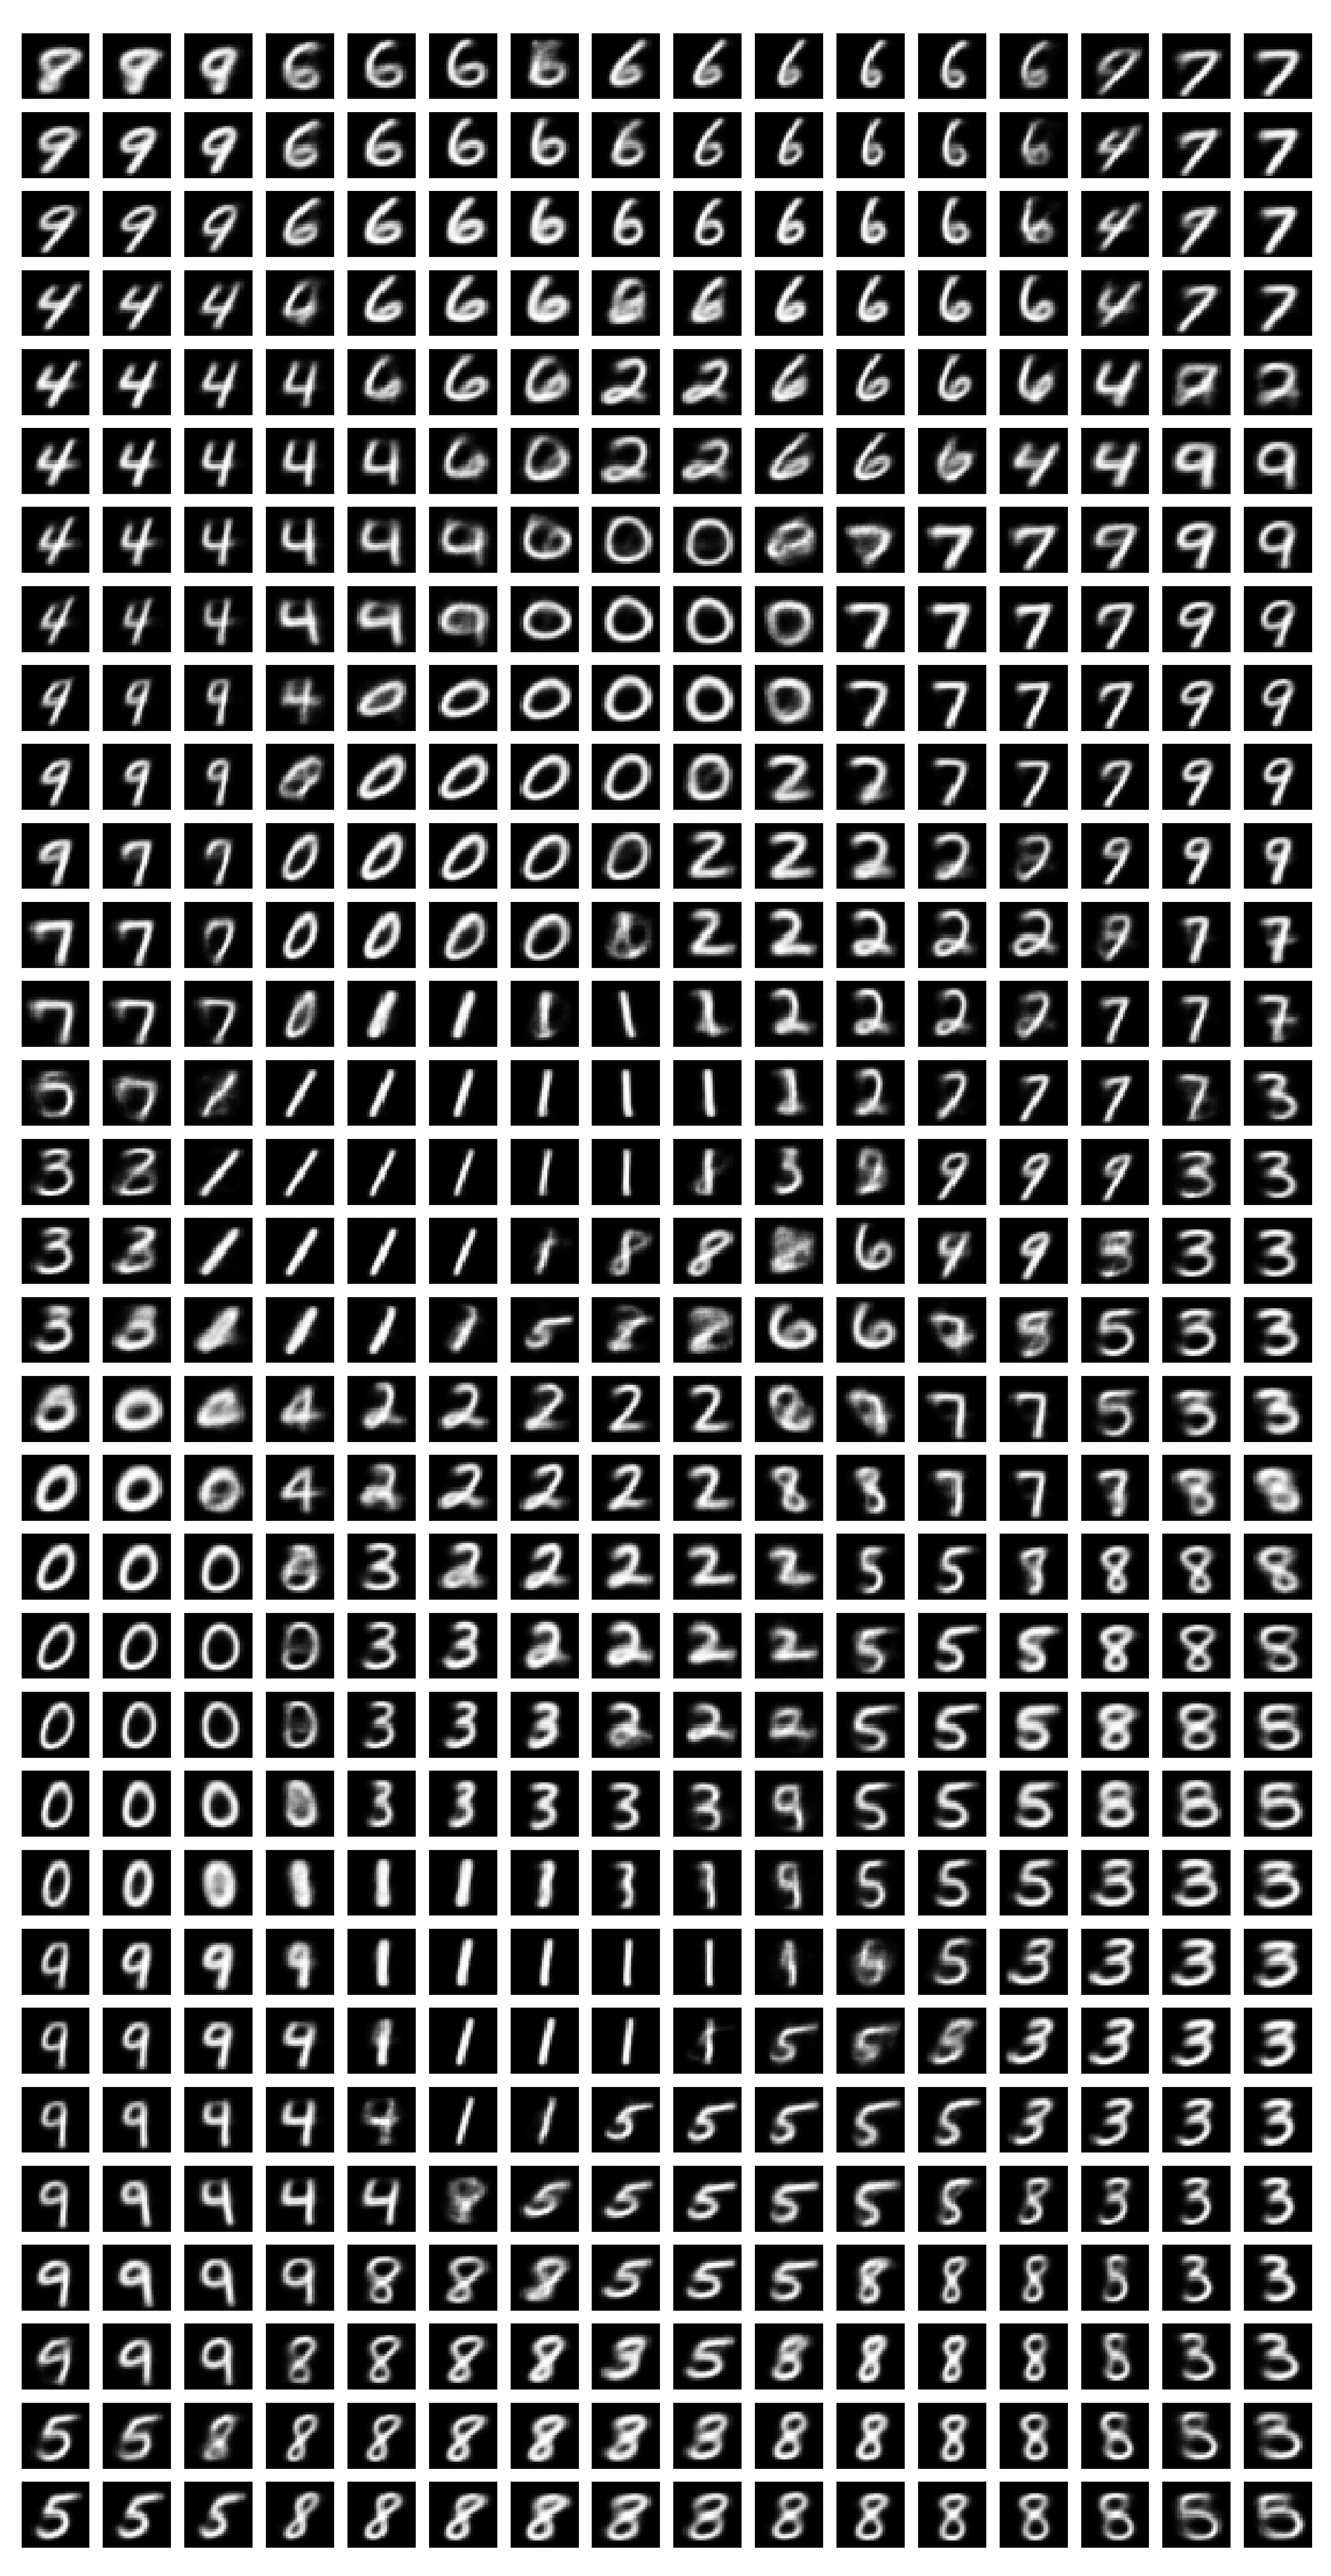
\includegraphics[height=0.8\textheight]{MNIST_SOM.pdf}
    \caption{Images generated from the SOM-VAE's latent space with 512 embeddings trained on MNIST. It yields an interpretable discrete two-dimensional representation of the data manifold in the higher-dimensional latent space.}
    \label{fig:MNIST_SOM}
\end{figure}

\begin{figure}[h]
    \centering
    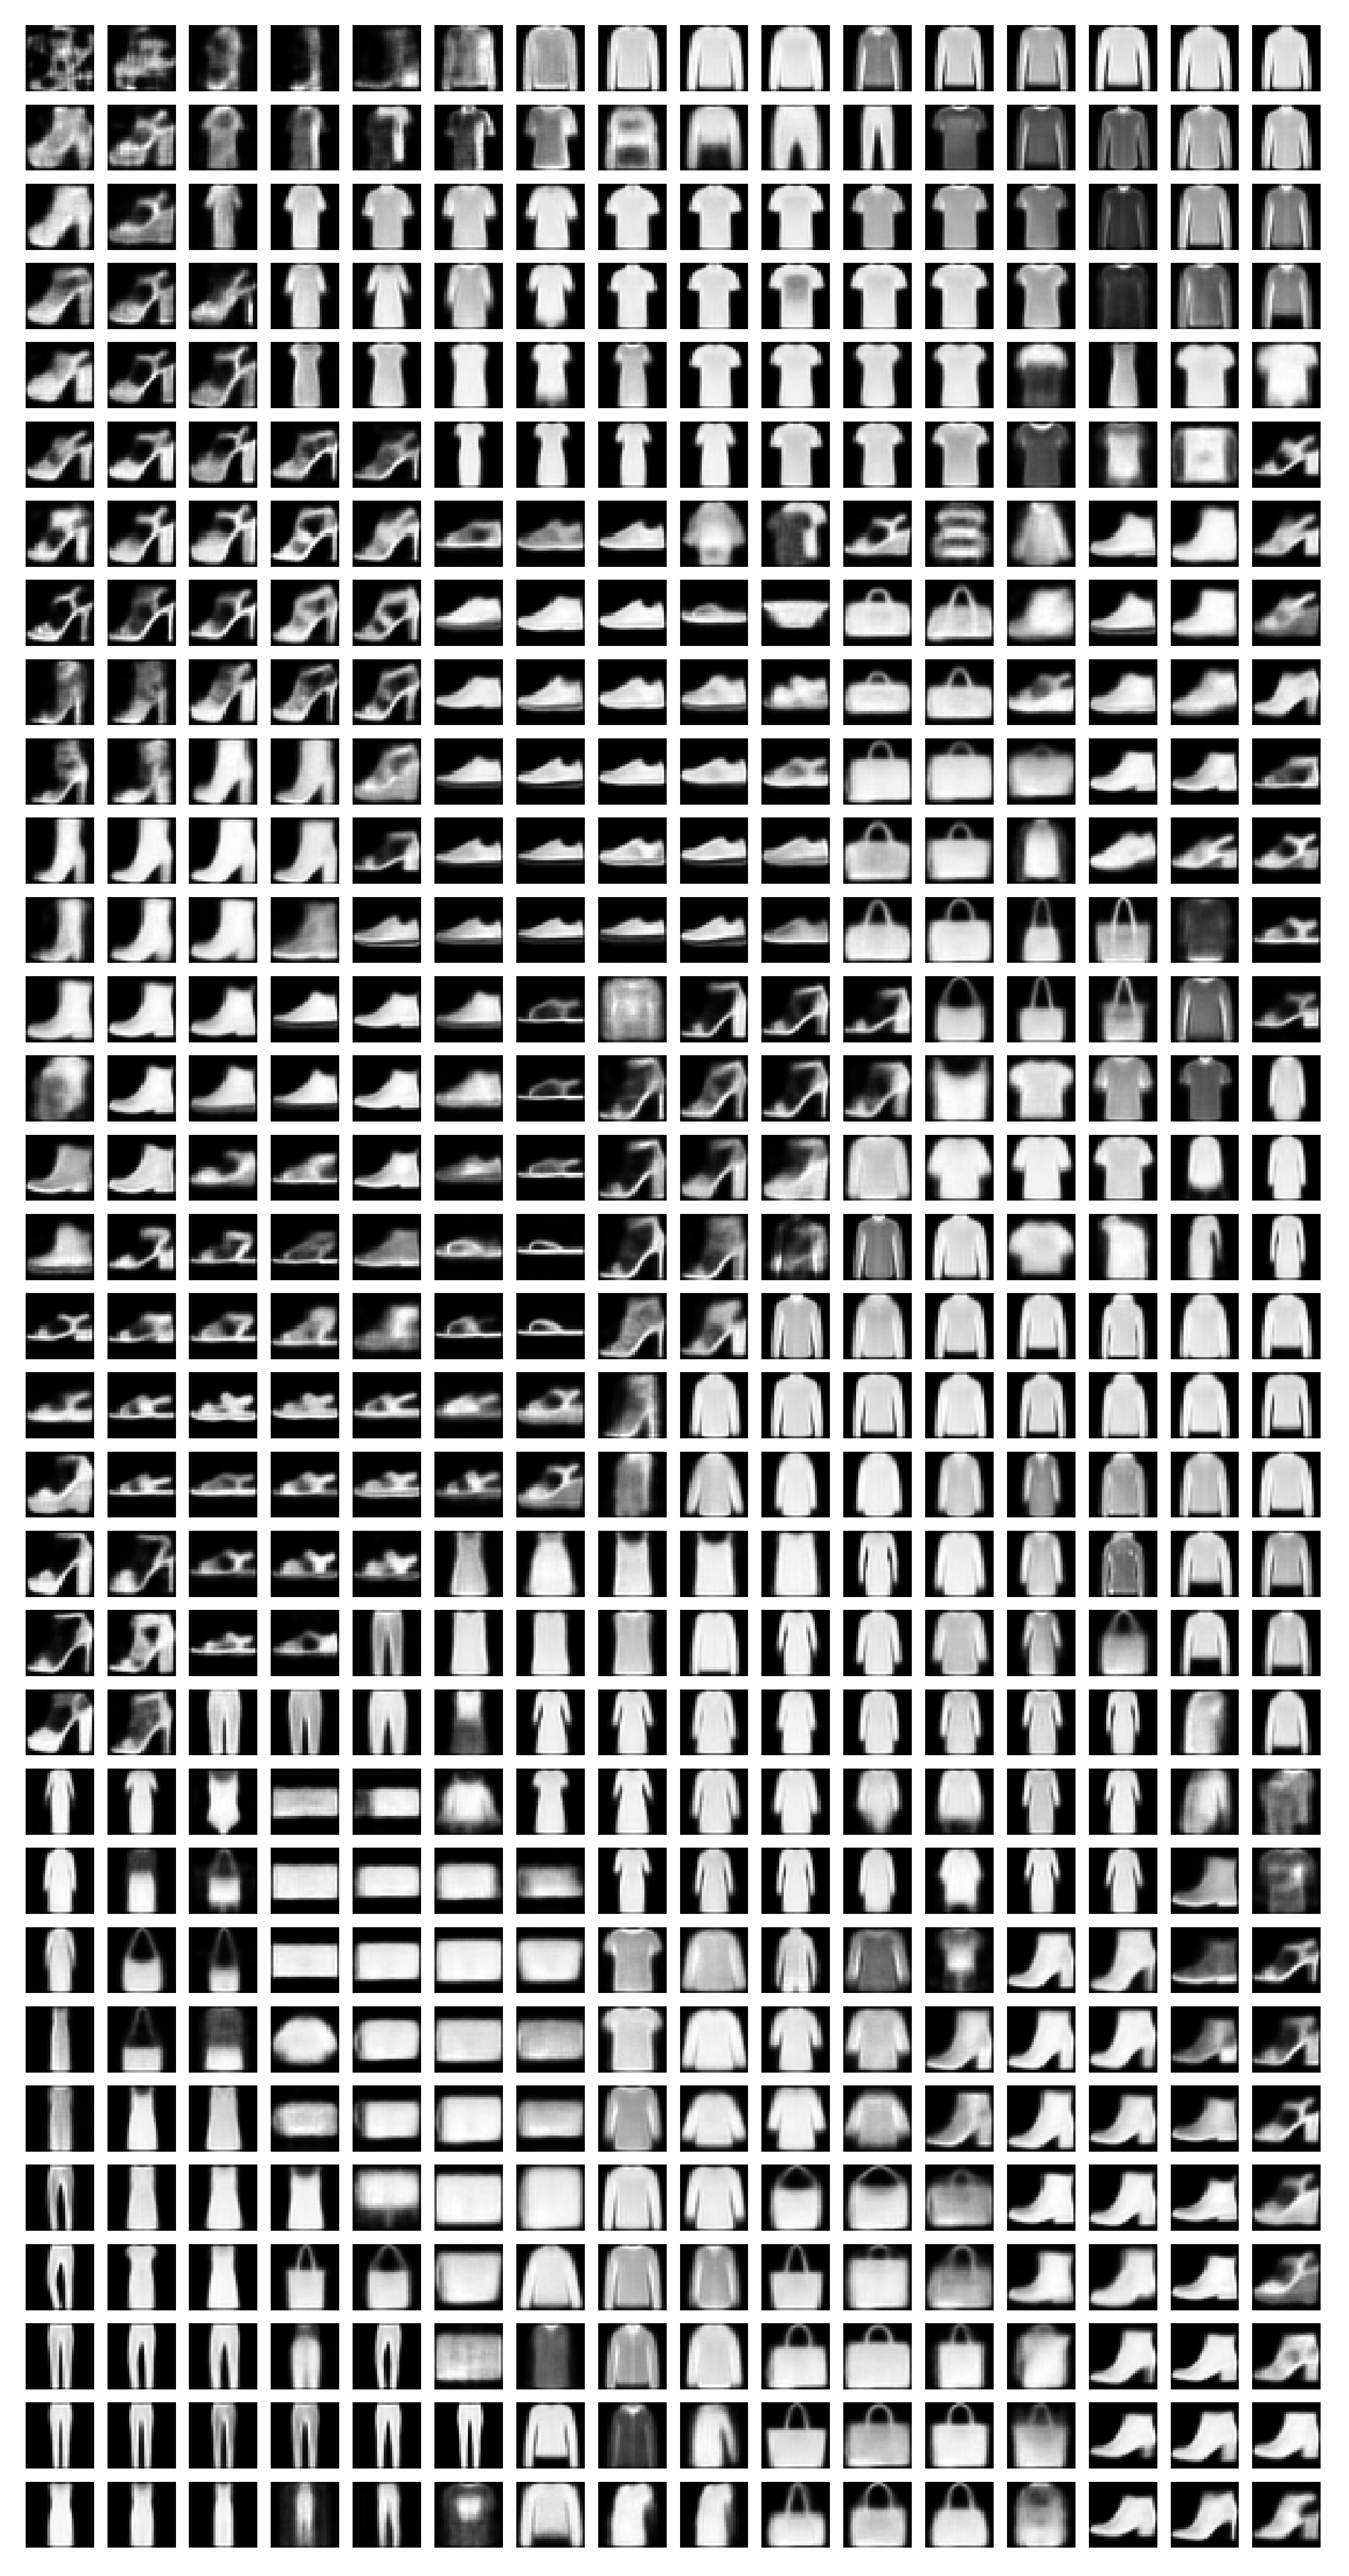
\includegraphics[height=0.8\textheight]{FMNIST_SOM.pdf}
    \caption{Images generated from the SOM-VAE's latent space with 512 embeddings trained on Fashion-MNIST. It yields an interpretable discrete two-dimensional representation of the data manifold in the higher-dimensional latent space.}
    \label{fig:FMNIST_SOM}
\end{figure}




